Para la generación de los resultados generamos 10 ejecuciones como las detalladas en la sección \textit{Desarrollo}.
Luego, generamos dos gráficos para analizar los valores de las muestras.

La figura \ref{modelo_shock_histo} describe la cantidad de celdas finales que
finalizaron la simulación siendo del partido \textit{A, B o I (indeciso)}.

Cada punto corresponde a una ejecución del experimento.



\begin{figure}[!h]
\centering
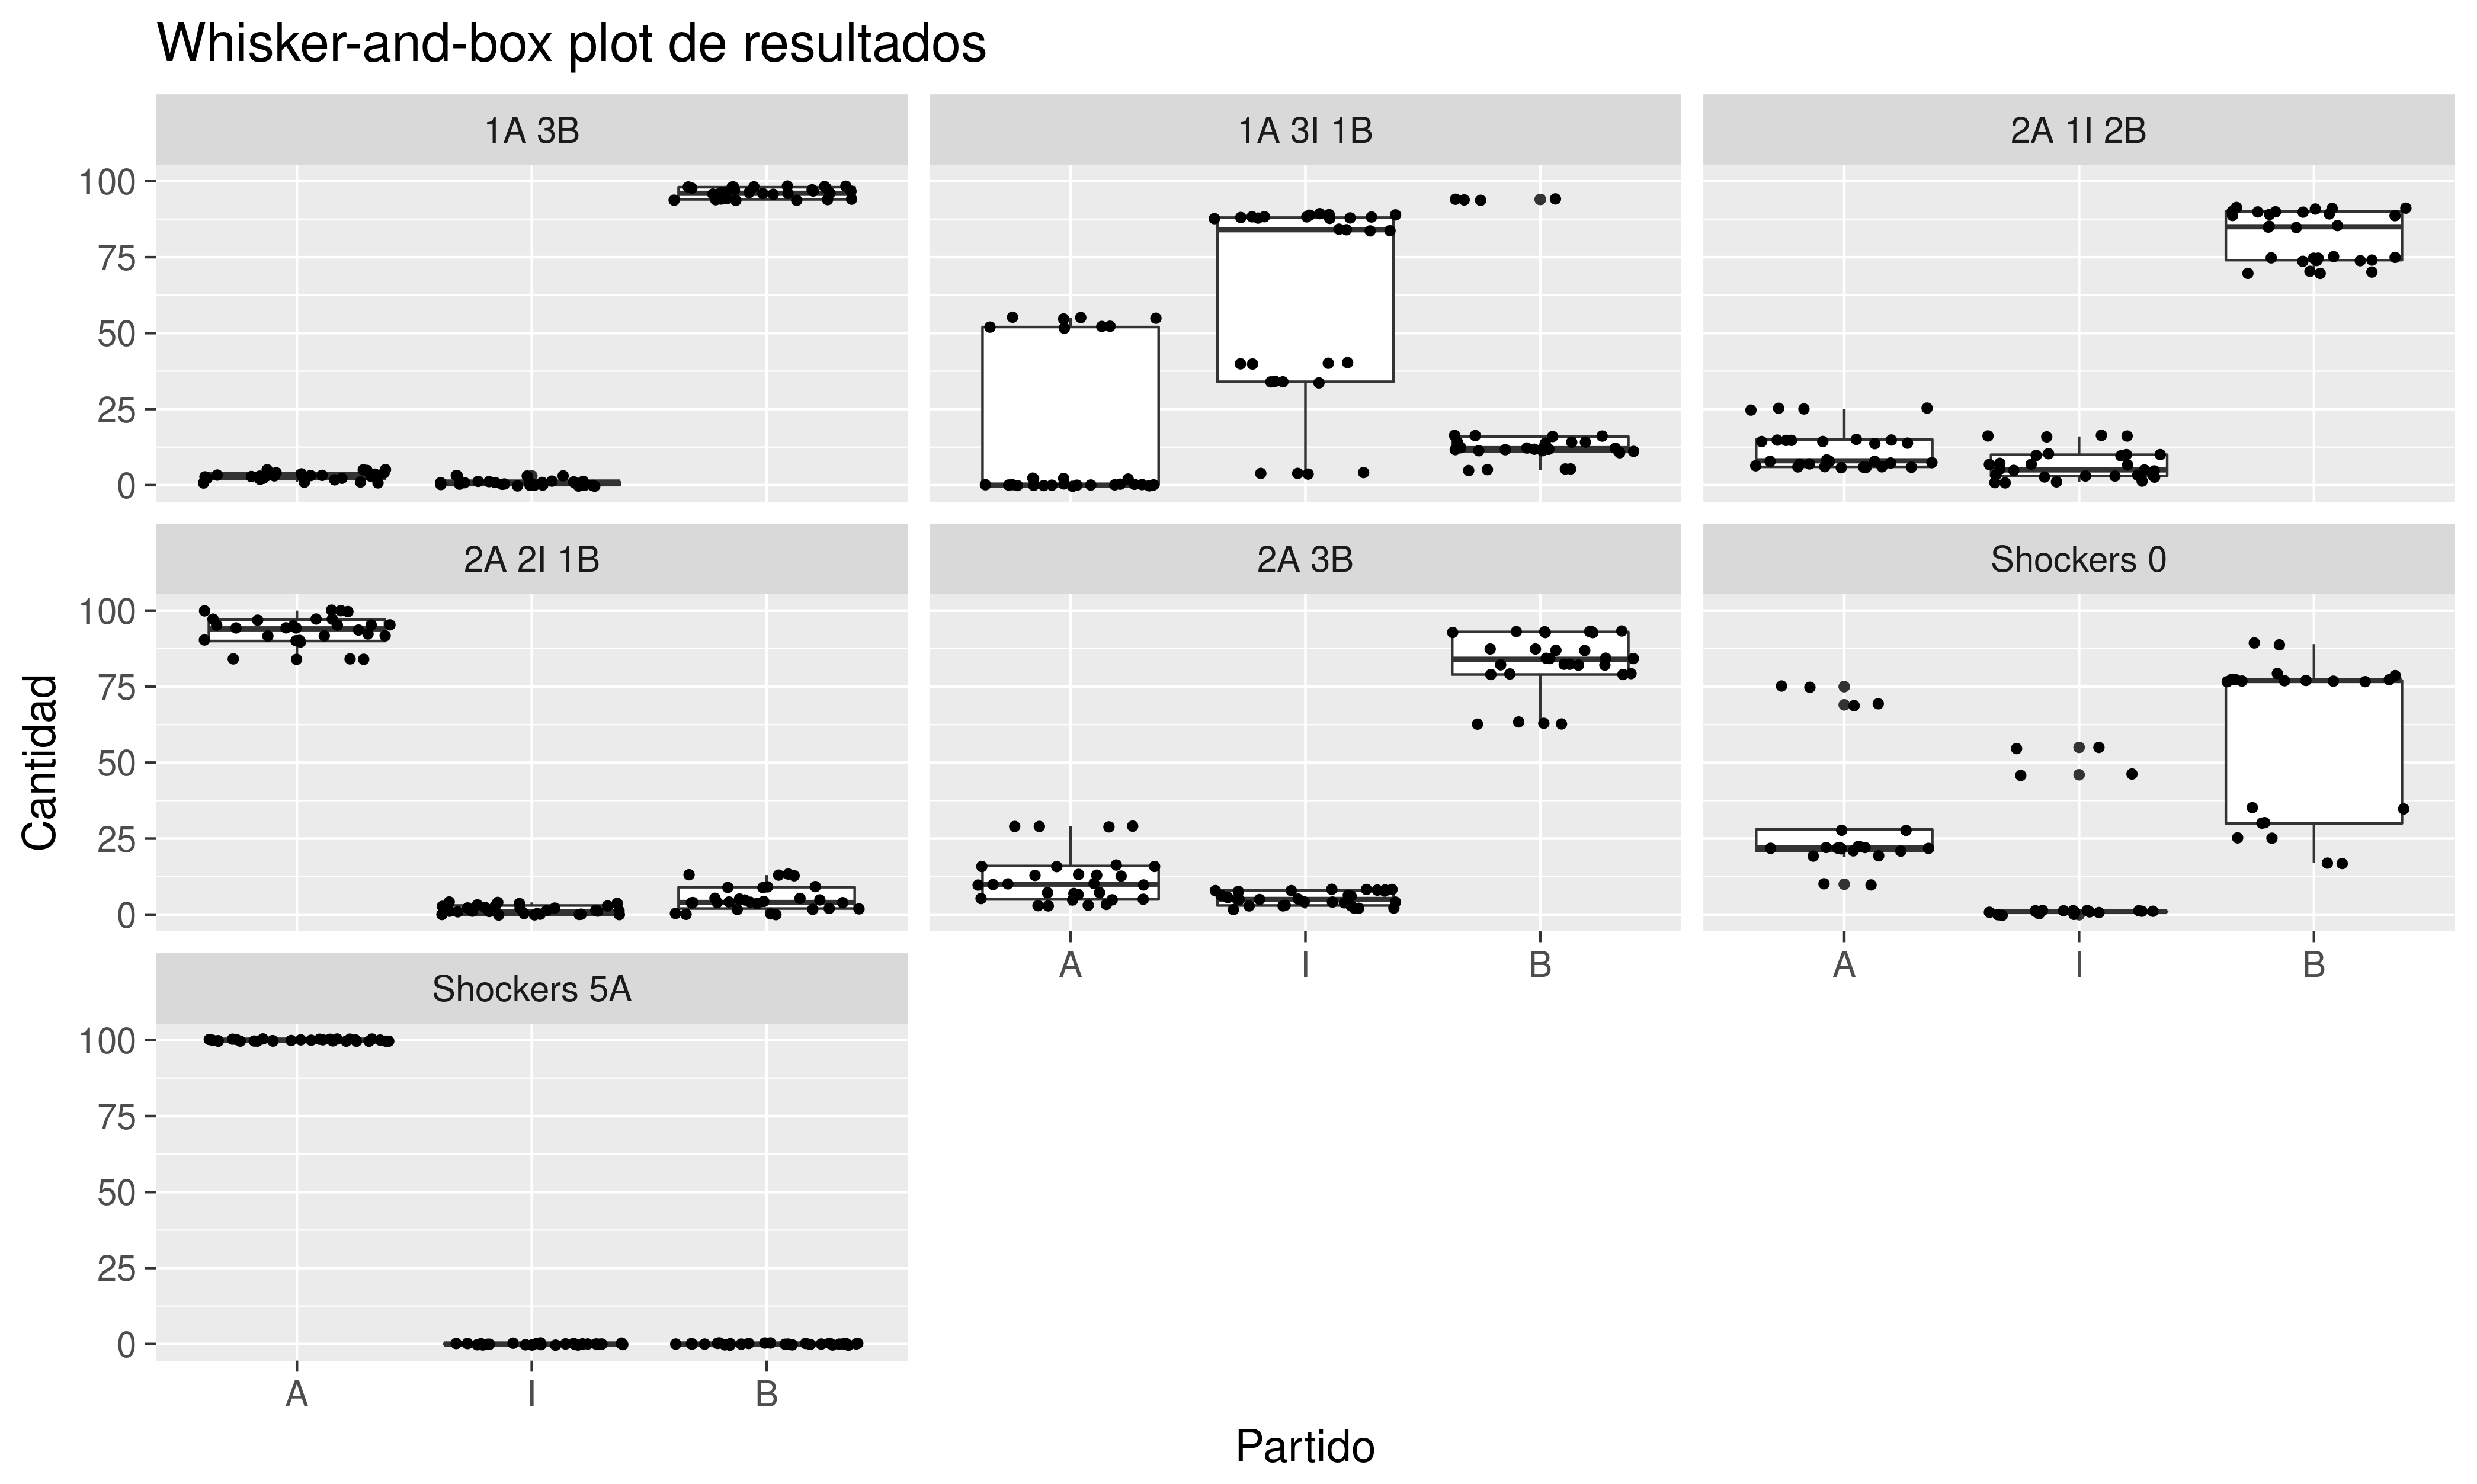
\includegraphics[scale=0.5]{imagenes/histograma_resultados.png}
\caption{Histograma para los resultados del modelo}
\label{fig:modelo_shock_histo}
\end{figure}

\begin{figure}[!h]
\centering
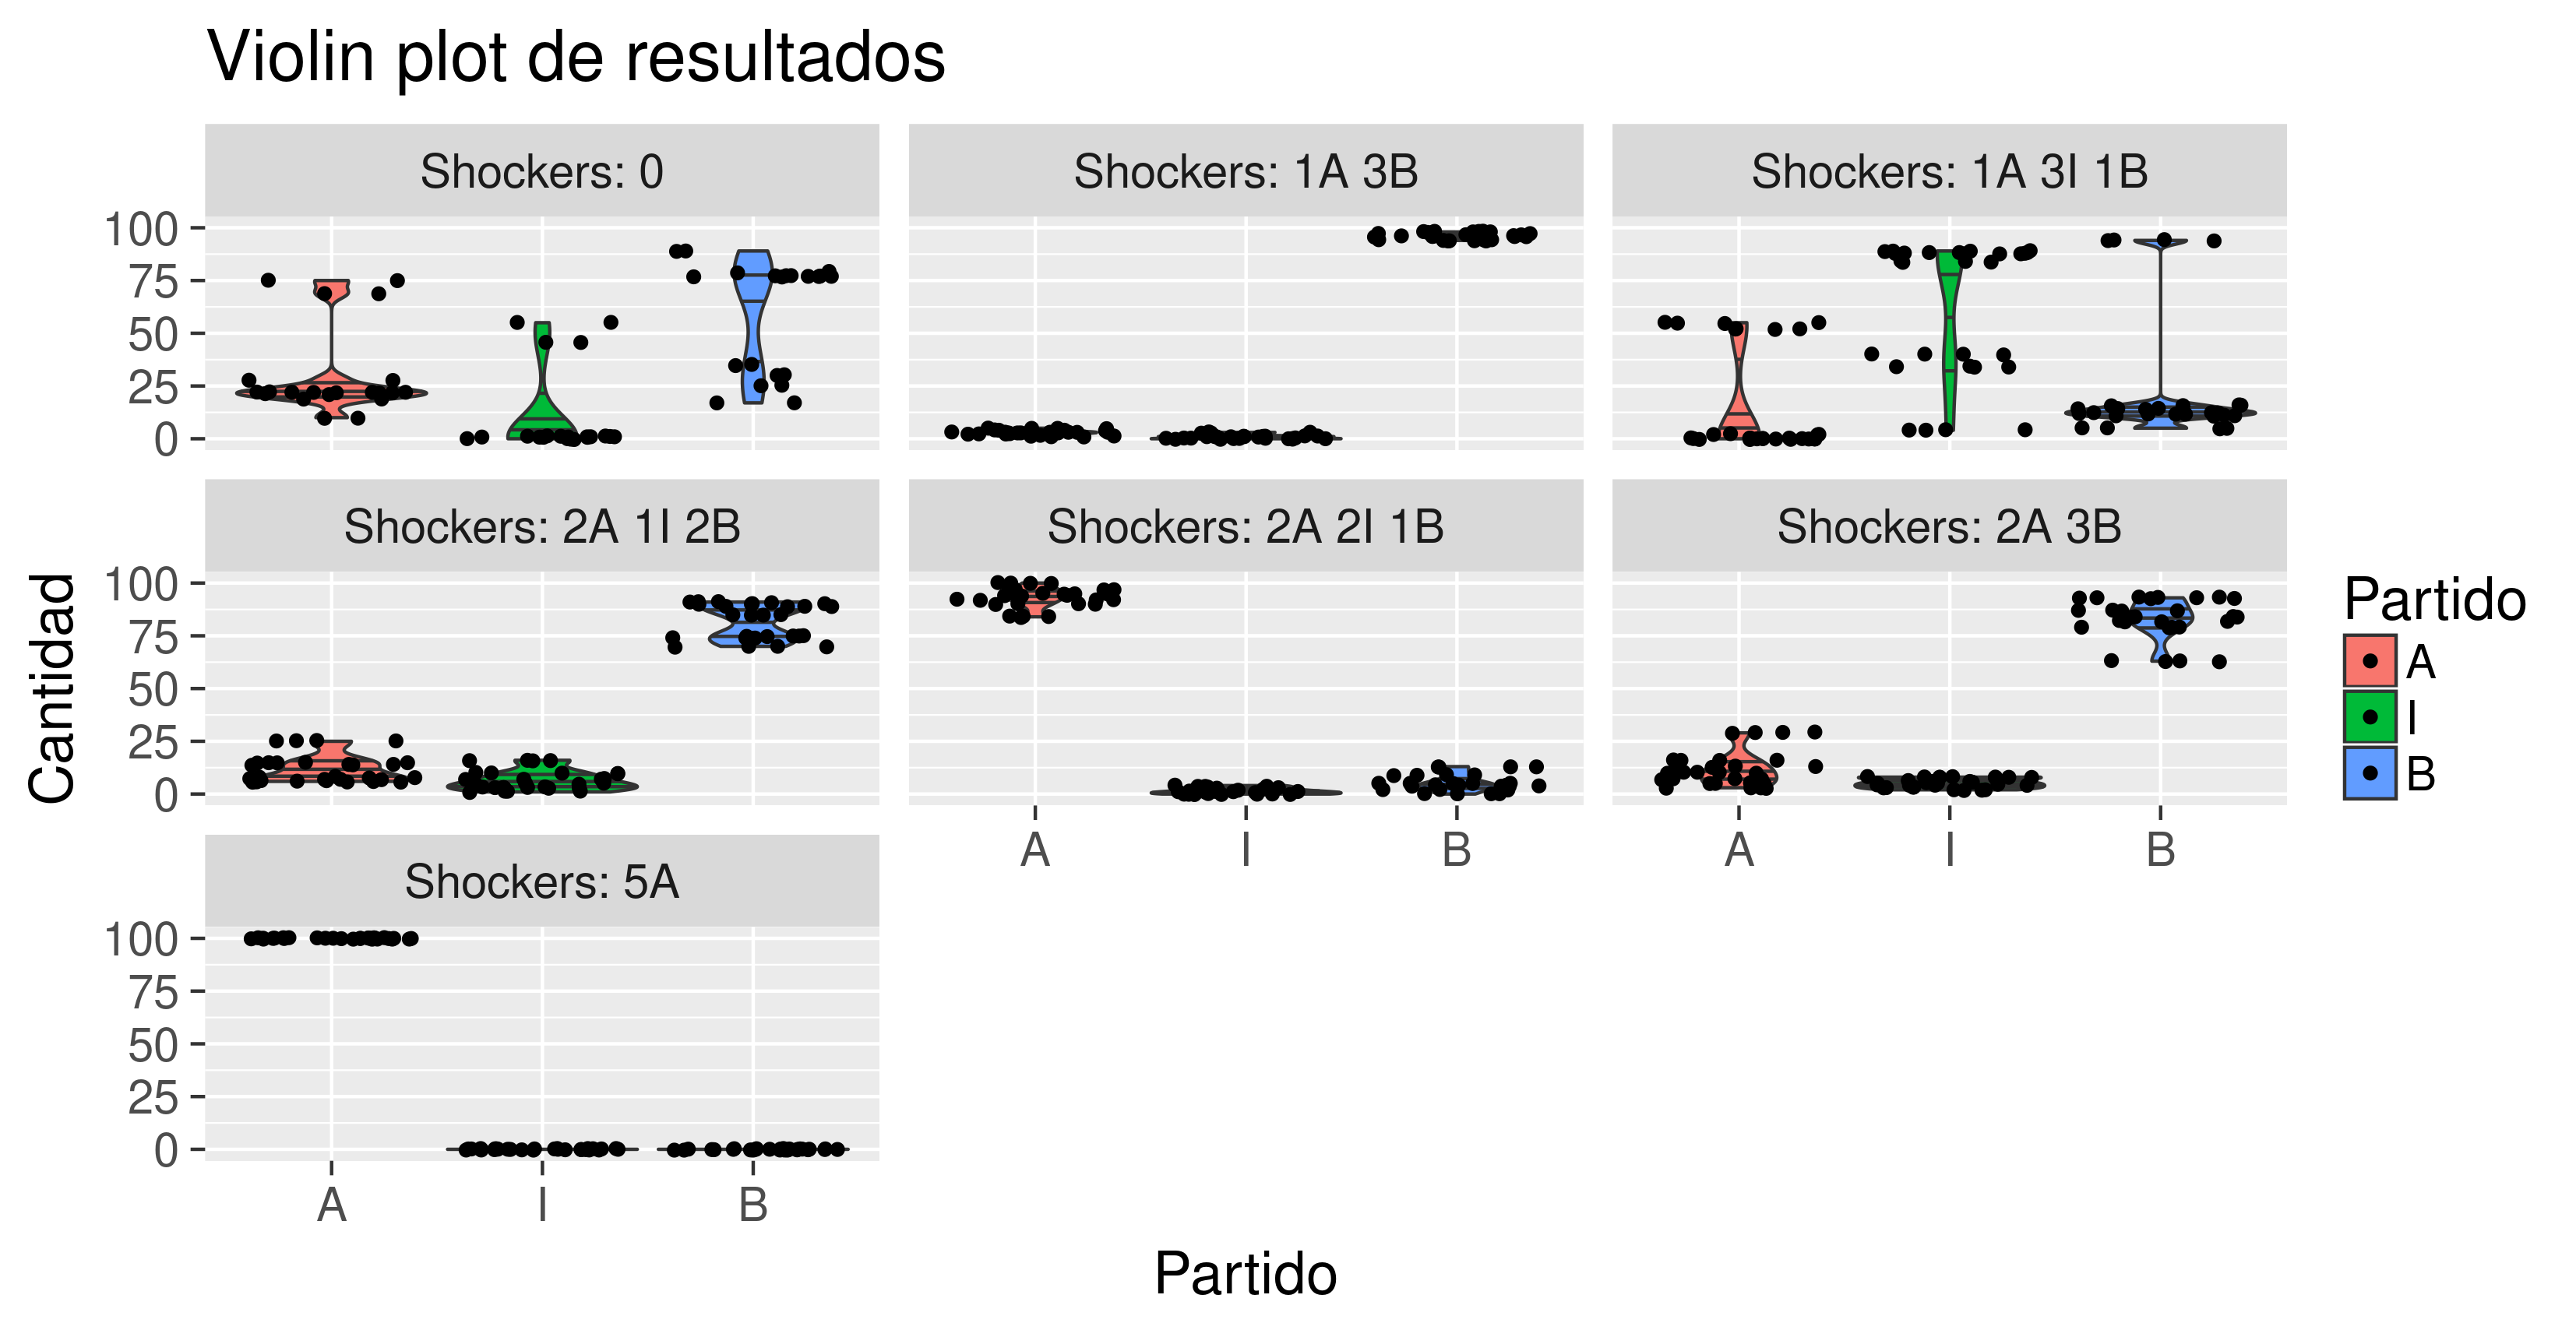
\includegraphics[scale=0.5]{/home/danito/facu/sed_2017/sed_2017_tps/tp2/informe/imagenes/violin_resultados.png}
\caption{Vecindario de celdas utilizado para definir el comportamiento de cada agente}
\label{fig:modelo_shock_violin}
\end{figure}
